% !TEX TS-program = xelatex
% !BIB program = bibtex
% !TeX spellcheck = ru_RU
% !TEX root = talk.tex

\documentclass
  [ russian
  , aspectratio=169 % Для защит онлайн лучше использовать разрешение не 4х3
  ] {beamer}


%%% Обязательные пакеты
%% Beamer
\usepackage{beamerthemesplit}
\usetheme{SPbGU}
\beamertemplatenavigationsymbolsempty
\usepackage{appendixnumberbeamer}

%% Локализация
\usepackage{fontspec}
\setmainfont{CMU Serif}
\setsansfont{CMU Sans Serif}
\setmonofont{CMU Typewriter Text}
%\setmonofont{Fira Code}[Contextuals=Alternate,Scale=0.9]
%\setmonofont{Inconsolata}
% \newfontfamily\cyrillicfont{CMU Serif}

\usepackage{polyglossia}
\setdefaultlanguage{russian}
\setotherlanguage{english}
\usepackage[autostyle]{csquotes} % Правильные кавычки в зависимости от языка

%% Графика
\usepackage{wrapfig} % Позволяет вставлять графику, обтекаемую текстом
\usepackage{pdfpages} % Позволяет вставлять многостраничные pdf документы в текст

%% Математика
\usepackage{amsmath, amsfonts, amssymb, amsthm, mathtools} % "Адекватная" работа с математикой в LaTeX

% Математические окружения с русским названием
\newtheorem{rutheorem}{Теорема}
\newtheorem{ruproof}{Доказательство}
\newtheorem{rudefinition}{Определение}
\newtheorem{rulemma}{Лемма}

%%% Дополнительные пакеты. Используются в презентации, но могут быть отключены при необходимости
\usepackage{tikz} % Мощный пакет для создание рисунков, однако может очень сильно замедлять компиляцию
\usetikzlibrary{decorations.pathreplacing,calc,shapes,positioning,tikzmark}

\usepackage{multirow} % Ячейка занимающая несколько строк в таблице

%% Пакеты для оформления алгоритмов на псевдокоде
\usepackage[noend]{algpseudocode}
\usepackage{algorithm}
\usepackage{algorithmicx}

\usepackage{fancyvrb}

\NewDocumentCommand{\xxHash}{}{\textsc{xxHash}}
\NewDocumentCommand{\riscv}{}{\textsc{RISC-V}}
\NewDocumentCommand{\xxh}{m}{\textsc{XXH{#1}}}
\NewDocumentCommand{\sew}{}{\textsc{SEW}}
\NewDocumentCommand{\vl}{}{\textsc{VL}}
\NewDocumentCommand{\rvv}{}{\textsc{RVV}}
\usepackage{booktabs}
\usepackage{tabularx}
\usepackage{siunitx} % для таблиц с единицами измерений

\setbeamertemplate{itemize items}[circle]
\setbeamertemplate{enumerate items}[circle]

\newcommand\blfootnote[1]{%
	\begingroup
	\renewcommand\thefootnote{}\footnote{#1}%
	\addtocounter{footnote}{-1}%
	\endgroup
}

\makeatletter

\input{pretitle.tex}
\input{title.tex}

\newcommand{\academicGroup}{\my@title@group@ru}
\newcommand{\advisorChair}{\my@title@chair@ru}
% То, что в квадратных скобках, отображается внизу по центру каждого слайда.
\title[Транслятор в Interaction Nets]{\my@title@title@ru}
% То, что в квадратных скобках, отображается в левом нижнем углу.
\author[\my@title@author@ru]{\my@title@author@ru, группа \academicGroup}
\institute[СПбГУ]{}
\date[13 марта 2025 г.]{}
\newcommand{\supervisor}{\my@title@supervisor@ru}
\newcommand{\supervisorPosition}{\my@title@supervisorPosition@ru}
\newcommand{\consultant}{\my@title@consultant@ru}
\newcommand{\consultantPosition}{\my@title@consultantPosition@ru}
\newcommand{\reviewer}{\my@title@reviewer@ru}
\newcommand{\reviewerPosition}{\my@title@reviewerPosition@ru}
\newcommand{\defenseYear}{\my@title@year@ru}

\makeatother
\begin{document}
{
\setbeamertemplate{footline}{}
% Лого университета или организации, отображается в шапке титульного листа
\begin{frame}
    \includegraphics[width=1.4cm]{figures/SPbGU_Logo.png}
    \vspace{-35pt}
    \hspace{-10pt}
    \begin{center}
        \begin{tabular}{c}
            \scriptsize{Санкт-Петербургский государственный университет} \\
            \scriptsize{\advisorChair}
        \end{tabular}
        \titlepage
    \end{center}

    \btVFill

    {\scriptsize
        % У научного руководителя должна быть указана научная степень
        \textbf{Научный руководитель:}  \supervisorPosition~\supervisor \\
        % Консультанта может и не быть. Должна быть указана должность или ученая степень
        % \textbf{Консультант:}  \consultantPosition~\consultant \\
        % Для учебной практики не обязателен. Должна быть указана должность или ученая степень
        % \textbf{Рецензент:} \reviewerPosition~\reviewer \\
        % TODO: добавить условие на включение рецензента в зависимости от вида отчета
    }
    \makeatother
    \begin{center}
        \vspace{5pt}
        \scriptsize{Санкт-Петербург\\ \defenseYear}
    \end{center}
\end{frame}
}

\begin{frame}{Введение}
    \begin{itemize}
        \item Задачи искусственного интеллекта и анализа графов естественным образом выражаются в терминах разреженной линейной алгебры
        \item Разреженная линейная алгебра влечёт за собой нерегулярный параллелизм $\implies$~требуются специализированные ускорители
        \item \INs{}~--- модель вычислений, допускающая параметризацию и в которой легко достигается параллелизм\footnote[frame]{Тут пока всё ещё большая дыра на тему параметризации в требованиях и экспериментах, которую я не понимаю, как легко объяснить}
        \item Существуют программные реализации \INs{}, однако попыток реализовать ускоритель на её основе пока не предпринималось
    \end{itemize}

\end{frame}

\begin{frame}{\Lamagraph{}}
    Проект \Lamagraph{} исследует возможности по разработке
    \begin{itemize}
        \item параметризуемого многоядерного сопроцессора для разреженной линейной алгебры на архитектуре \INs{}
        \item ML-подобного функционального языка программирования для программирования сопроцессора
    \end{itemize}
\end{frame}

\begin{frame}{Требования к проекту}
    К проекту выдвинуты следующие требования
    \begin{itemize}
        \item Параметризация всех компонентов типами агентов сети и правилами их редукции
        \item Возможность сбора статистики
        \item Возможность постановки сравнительных экспериментов
        \item Использование единого стека технологий~--- гомогенность
        \item Получение полнофункционального прототипа, содержащего все компоненты,важнее, чем детальная проработка какого-то отдельного компонента
        \item Расширяемость и модифицируемость
    \end{itemize}
\end{frame}

\begin{frame}{Общая структура проекта}
    \begin{center}
        \includegraphics[width=\linewidth]{figures/lamagraph-big-horiz.pdf}
    \end{center}
\end{frame}

% Обязательный слайд: четкая формулировка цели данной работы и постановка задачи
% Описание выносимых на защиту результатов, процесса или особенностей их достижения и т.д.
\begin{frame}
    \frametitle{Постановка задачи}
    \textbf{Целью} работы является разработка транслятора модельного функционального языка в \INs{}
    \vspace{1em}

    \textbf{Задачи}:
    \begin{enumerate}
        \item Реализовать интерпретатор модельного ML-подобного языка
              \begin{enumerate}
                  \item Конкретный синтаксис языка
                  \item AST и синтаксический анализатор
                  \item Алгоритм вывода типов
                  \item Рассахаривание в обогащенное $\lambda$-исчисление
                        \setbeamercolor{local structure}{fg=gray}
                  \item Интерпретатор обогащенного $\lambda$-исчисления
              \end{enumerate}
              \setbeamercolor{local structure}{fg=gray}
        \item Реализовать транслятор из обогащенного $\lambda$-исчисления в \INs{}
              %   \begin{enumerate}
              %       \item Представление набора агентов и правил редукции
              %       \item Сопоставление $\lambda$-термам соответствующих агентов
              %       \item Готовые наборы агентов и правил редукции
              %   \end{enumerate}
        \item Реализовать интерпретатор \INs{}
              %   \begin{enumerate}
              %       \item Последовательные редукции
              %       \item Последовательное исполнение параллельных редукций
              %       \item Сбор статистики с учётом способа редукции
              %   \end{enumerate}
        \item Провести эксперименты с наборами инструкций
    \end{enumerate}
    % \setbeamercolor{local structure}{fg=beamer@blendedblue}
\end{frame}

\begin{frame}{Архитектура транслятора}
    \begin{columns}
        \begin{column}{0.6\textwidth}
            \begin{itemize}
                \item Транслятор реализован на \Haskell{}
                \item Синтаксис основан на \OCaml{}; для представления AST используется Trees That Grow
                \item Парсер реализован с помощью связки \textsc{Alex} и \textsc{Happy} с применением property-based тестов
                \item Используется система типов Хиндли-Милнера
                \item Для упрощения дальнейших преобразований используется промежуточное представление~--- обогащенное $\lambda$-исчисление %в виде $\lambda$-исчисления обогащенного примитивными операциями, let-связываниями и сопоставлением с образом
            \end{itemize}
        \end{column}
        \begin{column}{0.35\textwidth}
            \begin{center}
                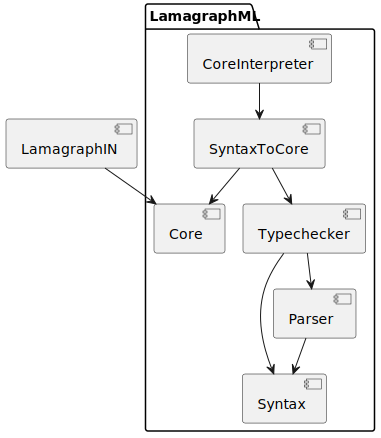
\includegraphics[width=\linewidth]{figures/components.pdf}
            \end{center}
        \end{column}
    \end{columns}
\end{frame}

\begin{frame}{План экспериментов}
    \begin{itemize}
        \item Существует не один способ трансляции $\lambda$-исчисления в \INs{}
        \item Планируется измерять для разных наборов агентов и правил редукции следующие метрики:
              \begin{itemize}
                  \item размер программы в терминах количества агентов
                  \item количество редукций
              \end{itemize}
        \item Поскольку \INs{} допускает параллельность также важны метрики:
              \begin{itemize}
                  \item максимальное количество одновременных (параллельных) редукций
                  \item количество шагов до достижения нормальной формы при неограниченном количестве параллельных редукций
              \end{itemize}
        \item Эксперименты планируется на операциях линейной алгебры, например умножении разреженных матриц в формате дерева квадрантов.
    \end{itemize}
\end{frame}

\begin{frame}
    \frametitle{Результаты}
    В рамках данной производственной практики были достигнуты следующие результаты\footnote[frame]{Исходный код находится в репозитории: \url{https://github.com/Lamagraph/interaction-nets-in-fpga} \\ Имя пользователя: \texttt{WoWaster}}
    \begin{enumerate}
        \item Реализована часть интерпретатора модельного ML-подобного языка
              \begin{enumerate}
                  \item Конкретный синтаксис языка
                  \item AST и синтаксический анализатор
                  \item Алгоритм вывода типов
                  \item Рассахаривание в обогащенное $\lambda$-исчисление
              \end{enumerate}
    \end{enumerate}
\end{frame}

\end{document}
